% !TeX root = ../main.tex

\subsection*{3.1 Step response}

1. Plotting the step response. The MATLAB script assumes $G(s) = \frac{1}{(s + 1)(0.5s + 1)} = \frac{1}{s + 1} \frac{1}{0.5s + 1}$ and $G_c(s) = \frac{-s + c}{c(s + 1)(0.5s + 1)} = \frac{-s + c}{c} \frac{1}{s + 1}\frac{1}{0.5s + 1}$.

\begin{figure}[H]
    \centering
    \begin{minipage}[t]{0.49\textwidth}
        \centering
        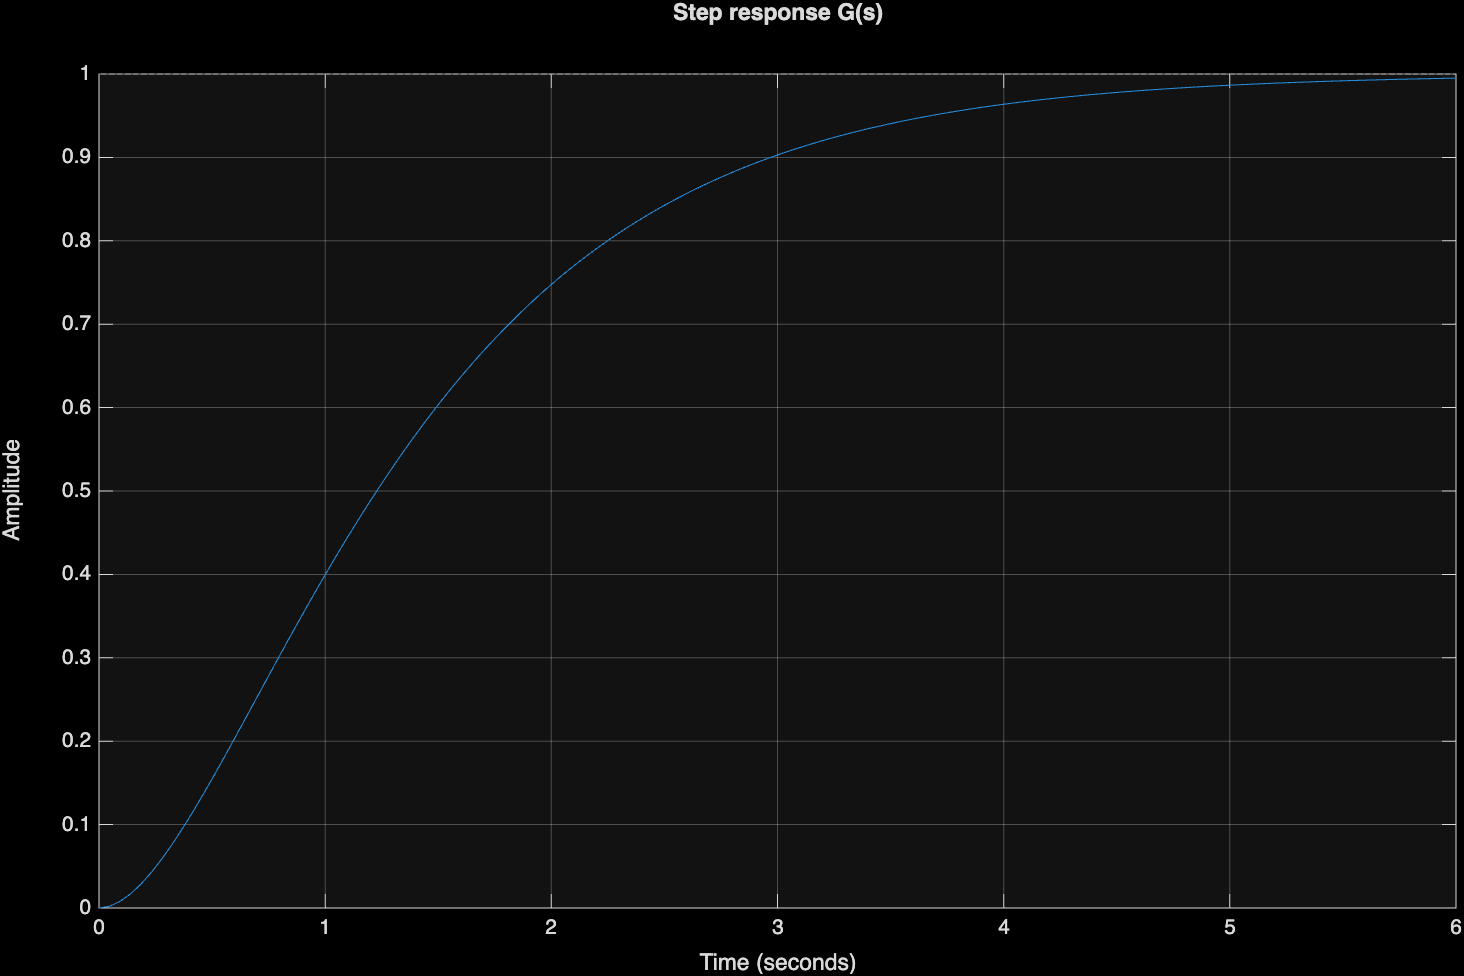
\includegraphics[width=\linewidth]{figures/3_1/g-step.png}
        \caption{Unit-step response of $G(s)$}
        \label{fig:g-step}
    \end{minipage}\hfill
    \begin{minipage}[t]{0.49\textwidth}
        \centering
        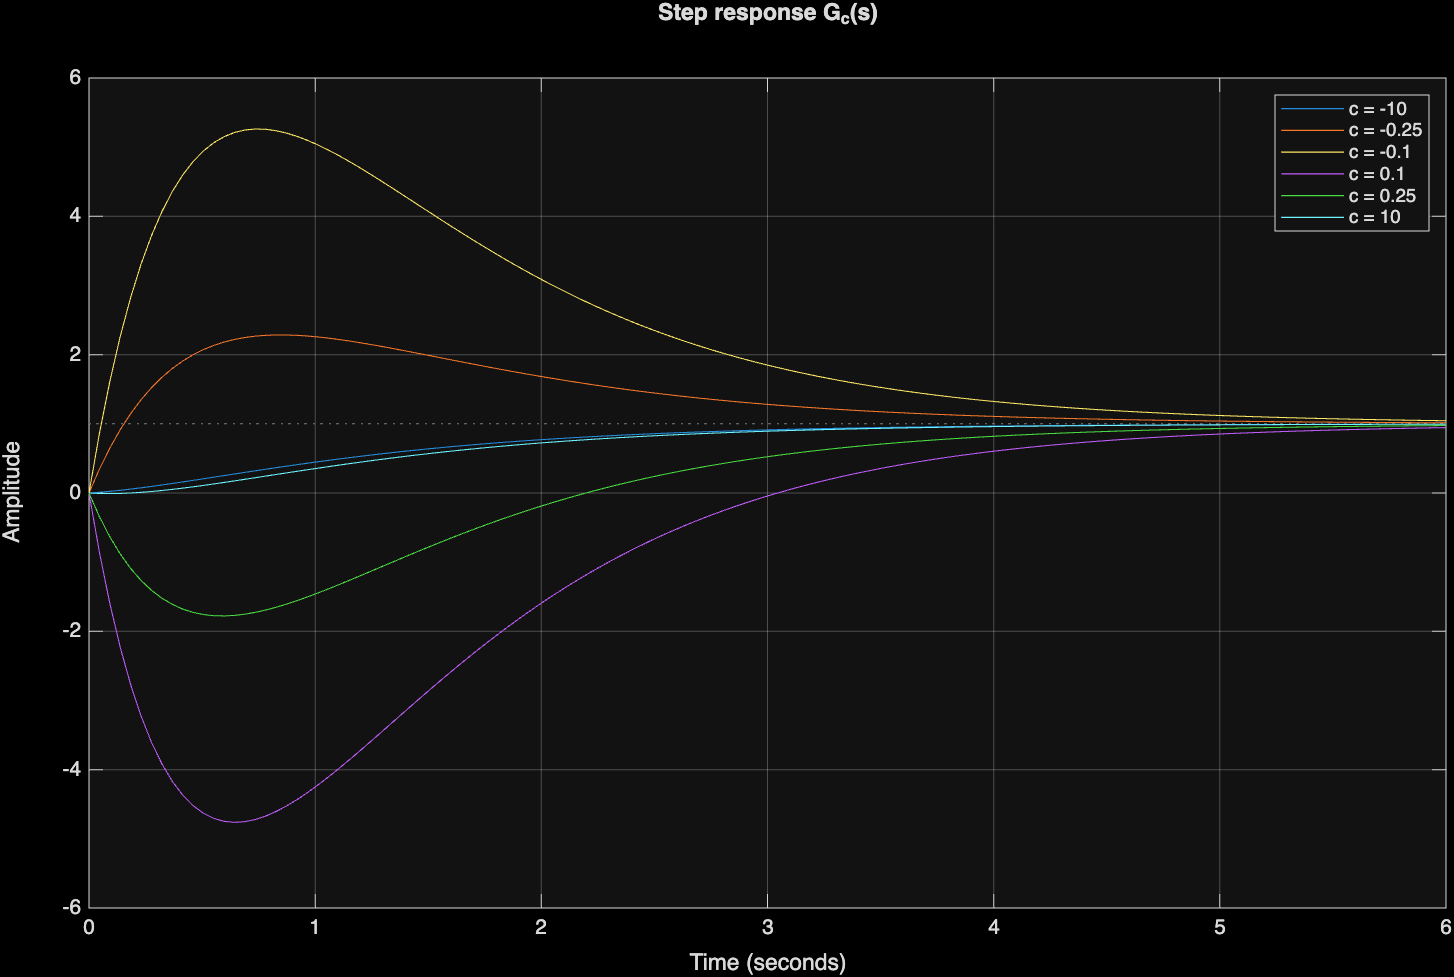
\includegraphics[width=\linewidth]{figures/3_1/g_c-step.png}
        \caption{Unit-step responses for different zero locations $c$.}
        \label{fig:g_c-step}
    \end{minipage}
\end{figure}

2. The overshoot and undershoot values are shown in the tables below.

\begin{table}[H]
    \centering
    \begin{minipage}[t]{0.49\textwidth}
    \centering
    \vspace{0pt}
    \small
    \pgfplotstabletypeset[
        col sep=comma,
        columns={Overshoot,Undershoot},
        fixed,
        fixed zerofill,
        precision=2,
        columns/Overshoot/.style={column name={Overshoot (\%)}},
        columns/Undershoot/.style={column name={Undershoot (\%)}},
        every head row/.style={
            before row=\toprule,
            after row=\midrule
        },
        every last row/.style={after row=\bottomrule}
    ]{tables/3_1/g-step-overshoot.csv}
    \caption{Overshoot and undershoot of $G(s)$.}
    \end{minipage}\hfill
    \begin{minipage}[t]{0.49\textwidth}
    \centering
    \vspace{0pt}
    \small
    \pgfplotstabletypeset[
        col sep=comma,
        columns={c,Overshoot,Undershoot},
        fixed,
        fixed zerofill,
        precision=2,
        columns/c/.style={column name={$c$}},
        columns/Overshoot/.style={column name={Overshoot (\%)}},
        columns/Undershoot/.style={column name={Undershoot (\%)}},
        every head row/.style={
            before row=\toprule,
            after row=\midrule
        },
        every last row/.style={after row=\bottomrule}
    ]{tables/3_1/g_c-step-overshoot.csv}
    \caption{Overshoot and undershoot of $G_c(s)$.}
    \end{minipage}
\end{table}

% p. 55 Second order systems, p. 57 Step response of second order systems
Writing $G(s)=\frac{2}{s^2+3s+2}$ in standard second-order form gives $\omega_n^2=2$ and $2\xi\omega_n=3$, hence $\xi=3/(2\sqrt{2})>1$. This is the second-order case with two real negative poles and no zero. Its unit-step response rises from~0 towards the final value~1, without oscillation, overshoot or undershoot.

% p. 44 Slow zeros and overshoot, p. 45,Effect of the zeros, an example
For $G_c(s)$ with $c<0$, the zero adds a temporary positive contribution while the original response is rising. For $c = -0.10$ and $c = -0.25$, it causes an overshoot. A zero close to the origin compared with the poles has a stronger effect, so $c=-0.1$ gives more overshoot than $c=-0.25$. At $c=-10$, the effect is too weak to cause overshoot.

% p. 40 Zeros, p. 44 Non minimum phase zeros and undershoot, p. 45, Effect of the zeros
For $G_c(s)$ with $c>0$, the zero adds a temporary negative contribution, so the response first falls before approaching the final value. This is the undershoot caused by a non minimum phase zero. Moving the zero closer to the origin increases its contribution. $c=0.1$ produces more undershoot than $c=0.25$, while $c=10$ produces only a small undershoot.
